            \documentclass[runningheads]{llncs}
%
% Springer LNCS format. On Overleaf: New Project > Templates > "Springer Lecture Notes in Computer Science",
% then replace main.tex and upload tables.tex, refs.bib, fig_scaling.pdf, fig_qual.png, fig_pareto.pdf, fig_uhd.png.
%
\usepackage[T1]{fontenc}
\usepackage{lmodern}
\usepackage{graphicx}
\usepackage{booktabs}
\usepackage{amsmath,amssymb}
\usepackage{multirow}
\usepackage{tikz}
\usetikzlibrary{positioning,arrows.meta,calc}
\usepackage{url}
\usepackage[hidelinks]{hyperref}
\renewcommand\UrlFont{\color{black}\rmfamily}

\begin{document}
\setlength{\emergencystretch}{3em}

\title{Enhance Small, Apply Large: An Empirical Study of Low-to-High-Resolution Transfer for HVI-CIDNet}
\titlerunning{Low-to-High-Resolution Transfer for HVI-CIDNet}

\author{Dao Thi Xuan Hieu \and Truong Kim Nguyen \and Nguyen Thien Huy}
\authorrunning{D. T. X. Hieu et al.}
\institute{Faculty of Information Technology, University of Science,\\
Vietnam National University Ho Chi Minh City, Vietnam\\
\email{\{25C12001, 25C12009, 25C12025\}@student.hcmus.edu.vn}}

\maketitle

\begin{abstract}
Low-light enhancement networks are trained and evaluated on small images, while phone cameras produce photographs of 8 to 48\,megapixels. Running such a network at full resolution is slow and memory-hungry on consumer hardware without a large GPU. We study how to reduce this cost for HVI-CIDNet without retraining: enhance a small copy of the image and transfer the result to the large one with an edge-aware affine transform fitted on a bilateral grid, in the spirit of bilateral guided upsampling. Our specific question is whether fitting this transform in the network's own HVI color space, instead of RGB, gives a better transfer. We compare a ladder of seven strategies, including overlapping tiling and a gain-aware denoising variant, against the full-resolution output of the same network, on the 100 test images of LOLv2-real (pseudo-high-resolution) and on 30 real $3840{\times}2160$ pairs of UHD-LL, with hyper-parameters frozen on LOLv2 training images. On both datasets the bilateral-grid transfer is much closer to the full-resolution output than bicubic upsampling (+3.0 to +3.4\,dB PSNR). Fitting in HVI does not help: on 4K images it differs from RGB by at most 0.04\,dB and is 3 to 6 times slower in the transfer step. The most important change with respect to small images concerns tiling: 512-pixel tiles are almost identical to the full-resolution output at $600{\times}400$ (42.8\,dB), but on real 4K images they drift far from it (18.8\,dB), whereas the transfer from a $1/8$ copy stays at 31.9\,dB and is closer to the full-resolution output than tiling on 27 of 30 images. A gain-aware denoising step smooths the amplified noise of the transfer but lowers fidelity to the network on both datasets. We report these mostly negative results together with code that regenerates every table.
\keywords{Low-light image enhancement \and HVI color space \and Bilateral guided upsampling \and High-resolution inference \and UHD-LL \and Reproducibility}
\end{abstract}

%------------------------------------------------------------------
\section{Introduction}
Low-light image enhancement turns dark, noisy photographs into well-exposed images. Recent networks reach strong results on small benchmark images, but phone cameras now produce 8 to 48\,megapixel (MP) photographs, and the networks were trained and evaluated on images of a few hundred pixels per side. HVI-CIDNet~\cite{hvicidnet} is a representative example. It converts the image into a learnable color space called HVI (hue, value, intensity), processes it with a two-branch network with cross attention, and converts it back. Its official evaluation uses $600{\times}400$ images, and its documentation does not discuss high-resolution inputs or memory.

Running such a network at full resolution is costly, and the cost matters most where users actually take photographs: laptops, phones and other devices without a large dedicated GPU. In our measurements (Section~\ref{sec:cost}), memory grows roughly linearly with the number of pixels; one forward pass at 10.8\,MP takes tens of seconds and about 25\,GB of memory, which exceeds what most consumer devices can provide. The practical question is therefore how to obtain an output close to the full-resolution result while running the network only on a small image. Two obvious workarounds exist: (i) cut the image into overlapping tiles, and (ii) run the network at low resolution and move the result to the full-resolution image. The second option has a long history in computational photography. Bilateral guided upsampling (BGU)~\cite{bgu} fits a locally affine color transform on a bilateral grid~\cite{bilateralgrid} from a low-resolution input/output pair and applies it to the full-resolution input, with no learning; HDRNet~\cite{hdrnet} replaces the fitting step with a network.

This paper is an empirical study, not a new method. We take an existing transfer technique (BGU) and an existing network (HVI-CIDNet) and measure how cheap pipelines compare with full-resolution inference in quality, time and memory. Within this study we ask one specific question: \emph{does it help to fit the transform in the HVI space of the network rather than in RGB?} The HVI space was designed so that brightness and chroma are decoupled and dark-region color noise is reduced, which suggests that an affine transform may be better conditioned there. We do not claim BGU as our contribution. Our contributions are:
\begin{itemize}
\item a reproduction of the released LOLv2-real checkpoint on consumer hardware without a CUDA GPU (Table~\ref{tab:repro});
\item a seven-rung ablation ladder of transfer strategies, evaluated against the full-resolution output of the network (the ``teacher'') and against ground truth, with paired significance tests, on pseudo-high-resolution LOLv2-real and on real 4K images of UHD-LL with hyper-parameters frozen in advance;
\item a measurement of memory and time for full-resolution, tiled and low-resolution pipelines at 8.3 and 10.8\,MP;
\item two negative results: fitting in HVI is not better than fitting in RGB, and a gain-aware denoising step does not improve fidelity; and one result that depends on image size: tiling, which is nearly exact at $600{\times}400$, is far from the full-resolution output at 4K, where the low-resolution transfer is the better cheap pipeline.
\end{itemize}

%------------------------------------------------------------------
\section{Related Work}
\paragraph{Low-light enhancement.} Retinex-based and end-to-end networks are evaluated mostly on LOL-style datasets~\cite{retinexnet,lolv2} with images of $600{\times}400$ pixels. HVI-CIDNet~\cite{hvicidnet} introduces the HVI color space and a lightweight cross-attention network (CIDNet) that works on the HV and I branches. The UHD-LL benchmark~\cite{uhdll} provides paired 4K low-light images; we use part of its test set to evaluate transfer on real high-resolution data, with a network trained on LOLv2.

\paragraph{Edge-aware transfer from low to high resolution.} Joint bilateral upsampling~\cite{jbu} and the guided filter~\cite{guided} upsample a low-resolution result using the full-resolution image as a guide. The bilateral grid~\cite{bilateralgrid} lifts the image into a (position, intensity) space in which smoothing is edge-aware. BGU~\cite{bgu} fits per-cell affine color transforms on such a grid from an input/output pair, and HDRNet~\cite{hdrnet} learns the transform with a network. Our work evaluates this family for a specific modern enhancement network and a specific color space.

%------------------------------------------------------------------
\section{Method}
\paragraph{Setting.} Let $f$ be the pretrained network and $I_{hr}$ the full-resolution input. The \emph{teacher} is $T=f(I_{hr})$. We downscale $I_{hr}$ by a factor $s$ with area averaging to obtain $I_{lr}$ and compute $O_{lr}=f(I_{lr})$. Each method builds an output $\hat O_{hr}$ from $(I_{hr},I_{lr},O_{lr})$ without further training. The goal is that $\hat O_{hr}$ approximates $T$ at a fraction of the cost (Fig.~\ref{fig:pipeline}).

\begin{figure}[t]
\centering
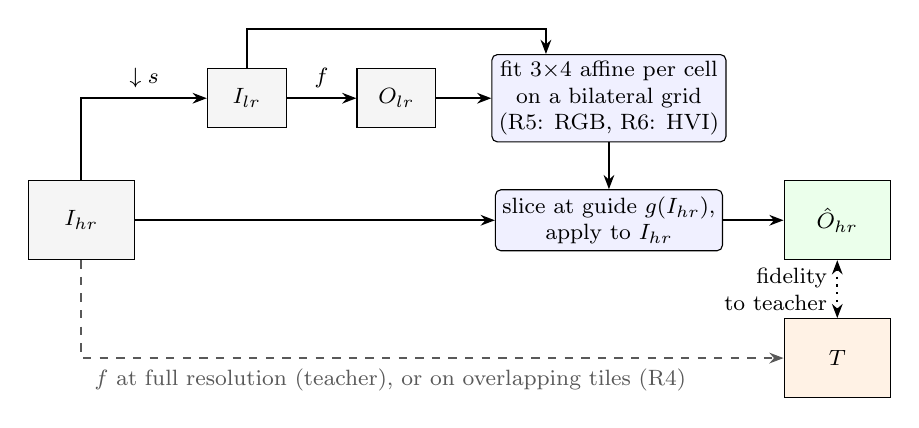
\begin{tikzpicture}[
  font=\footnotesize, >={Stealth[length=1.8mm]},
  img/.style={draw, minimum width=1.0cm, minimum height=0.75cm, fill=gray!8},
  big/.style={img, minimum width=1.35cm, minimum height=1.0cm},
  op/.style={draw, rounded corners=2pt, align=center, fill=blue!6, inner sep=2.5pt},
  cheap/.style={->, thick},
  costly/.style={->, thick, dashed, gray!70!black}]
\node[big] (Ihr) at (0,0) {$I_{hr}$};
\node[img] (Ilr) at (2.1,1.55) {$I_{lr}$};
\node[img] (Olr) at (4.0,1.55) {$O_{lr}$};
\node[op] (fit) at (6.7,1.55) {fit $3{\times}4$ affine per cell\\on a bilateral grid\\(R5: RGB, R6: HVI)};
\node[op] (apply) at (6.7,0) {slice at guide $g(I_{hr})$,\\apply to $I_{hr}$};
\node[big, fill=green!8] (Ohat) at (9.6,0) {$\hat O_{hr}$};
\node[big, fill=orange!10] (T) at (9.6,-1.75) {$T$};
\draw[cheap] (Ihr.north) |- node[pos=0.75, above] {$\downarrow s$} (Ilr.west);
\draw[cheap] (Ilr) -- node[above] {$f$} (Olr);
\draw[cheap] (Olr) -- (fit);
\draw[cheap] (Ilr.north) -- ++(0,0.5) -| ($(fit.north)+(-0.8,0)$);
\draw[cheap] (fit) -- (apply);
\draw[cheap] (Ihr) -- (apply);
\draw[cheap] (apply) -- (Ohat);
\draw[costly] (Ihr.south) |- node[pos=0.72, below] {$f$ at full resolution (teacher), or on overlapping tiles (R4)} (T.west);
\draw[<->, thick, dotted] (Ohat) -- node[left, align=right] {fidelity\\to teacher} (T);
\end{tikzpicture}
\caption{Low-to-high-resolution transfer. Solid arrows: the cheap pipeline, in which the network $f$ runs only on the $1/s$ copy and a bilateral-grid affine transform fitted from $(I_{lr},O_{lr})$ is applied to $I_{hr}$. Dashed arrow: the expensive alternatives, full-resolution inference (the teacher $T$) and tiling. Methods are compared by their fidelity to $T$ and by their quality against ground truth.}
\label{fig:pipeline}
\end{figure}


\paragraph{Transfer strategies (ablation ladder).} We use the following rungs.
\begin{description}
\item[R1] Bicubic upsampling of $O_{lr}$.
\item[R2] Per-channel gain ratio $g=(O_{lr}+\epsilon)/(I_{lr}+\epsilon)$ with $\epsilon=0.02$, upsampled (bicubic, R2; or then smoothed with a guided filter, R2$'$) and multiplied into $I_{hr}$.
\item[R3] Guided-filter upsampling~\cite{guided} of $O_{lr}$, with a log-scaled $I_{hr}$ as the guide.
\item[R4] Overlapping tiling: $f$ is run on tiles of $t{\times}t$ pixels with overlap $t/4$ and feathered (linear-ramp) blending. This needs no low-resolution pass.
\item[R5] Affine transform on a bilateral grid in RGB (next paragraph).
\item[R6] The same affine transform in the HVI space of the network.
\item[R7] R5 applied to a locally denoised input (end of this section).
\end{description}
R4 is not a transfer method, but it is the obvious alternative when an image does not fit in memory, so it belongs in the comparison.

\paragraph{Bilateral-grid affine transform (R5, R6).} We use our own simplified re-implementation of the idea of BGU~\cite{bgu}; it is not the authors' solver. Let $x$ be the source (input) and $y$ the destination (network output) at low resolution, both with three channels. The grid has axes (column, row, guide) with spatial cell size $\sigma_s$ low-resolution pixels and $n_b$ bins along the guide. The guide is the log-scaled maximum channel of the input,
\begin{equation}
g=\frac{\log(m+\delta)-\log\delta}{\log(1+\delta)-\log\delta},\quad m=\max_c x_c,\ \delta=10^{-3},
\end{equation}
which spreads the dark values over the guide range. Every low-resolution pixel is splatted trilinearly into the grid, accumulating $\sum \tilde x\tilde x^\top$ and $\sum y\tilde x^\top$ with $\tilde x=[x;1]$. The grid is smoothed with a $[1,2,1]$ kernel along all three axes, and each cell solves a $3{\times}4$ affine matrix by ridge regression toward the global least-squares fit (weight $\lambda$ per unit of cell mass). At full resolution the matrices are sliced trilinearly at (column, row, guide of $I_{hr}$) and applied to $I_{hr}$.

For R6 the same procedure runs in the HVI space of the network. The source is the HVI transform of the input and the destination is the HVI-space output of the network just before its inverse transform (this includes the network's residual connection). The result is converted back with the inverse HVI transform of the network. The guide is the log-scaled I channel, which is identical to the guide used in R5, so R5 and R6 differ only in the color space of the fit.

\paragraph{Gain-aware denoising (R7).} R5 applies the fitted transform to the noisy input $I_{hr}$, so input noise in dark regions is multiplied by the local gain, whereas the network removes it. R7 tries to compensate for this without training. A denoised copy $D_{hr}$ of $I_{hr}$ is computed with a self-guided guided filter (radius $r$, regularization $\epsilon_d$). The local gain is estimated at low resolution as $G=(\bar O_{lr}+0.02)/(\bar I_{lr}+0.02)$, where the bar denotes the channel mean, and upsampled bicubically. The transform fitted exactly as in R5 is then applied to $(1-w)\,I_{hr}+w\,D_{hr}$ with $w=\mathrm{clip}((G-g_0)/(g_1-g_0),0,1)$, so only strongly brightened regions are denoised. The guide for slicing is still computed from $I_{hr}$.

%------------------------------------------------------------------
\section{Experimental Setup}
\paragraph{Data.} We use LOLv2-real~\cite{lolv2}: 100 test pairs for all reported results, and 689 training pairs only for selecting hyper-parameters. Images are $600{\times}400$. This is a pseudo-high-resolution protocol: the full-size image plays the role of $I_{hr}$ and downscaling by $s\in\{2,4,8\}$ gives $I_{lr}$ (so the network sees $300{\times}200$, $150{\times}100$ or $75{\times}50$ inputs). For real high-resolution data we use the UHD-LL test set~\cite{uhdll} (150 pairs of $3840{\times}2160$, 8.3\,MP). Because one full-resolution teacher pass takes about 20\,GB and the whole ladder about 4 minutes per image on our machine, we evaluate a subset of 30 pairs (every 5th of the test pairs sorted by name), fixed before any result was computed. UHD-LL is used only for testing: all hyper-parameters are those frozen on LOLv2 training images, and the network has never seen UHD-LL images.

\paragraph{Network.} We use the released LOLv2-real \texttt{best\_PSNR} checkpoint of HVI-CIDNet with the configuration of the official evaluation script (\texttt{gated2}=true, $\alpha=0.8$, $\gamma=1$) and no ground-truth-mean rescaling (\texttt{use\_GT\_mean}=false) anywhere. The network is never retrained or fine-tuned.

\paragraph{Metrics.} Outputs are quantized to 8 bits and evaluated with the metric code of the official repository (PSNR; SSIM~\cite{ssim} with a Gaussian window as in the MATLAB implementation; LPIPS with AlexNet~\cite{lpips}). We report two families of numbers: fidelity to the teacher (PSNR, SSIM of $\hat O_{hr}$ against $T$), which measures how well a cheap pipeline approximates the expensive one, and quality against the ground truth (PSNR, SSIM, LPIPS). Differences between methods are tested on per-image paired values with the Wilcoxon signed-rank test.

\paragraph{Hyper-parameter selection.} Hyper-parameters were selected only on 30 training images (every 23rd of the 689 pairs), by mean PSNR to the teacher at $\times2$ and $\times4$, and frozen before evaluating on the test set. For the guided filter we searched radius $\in\{1,2,4,8,16\}$ and $\epsilon\in\{10^{-4},\dots,0.1\}$ (selected: radius 1, $\epsilon=0.01$). For the bilateral grid we first selected one shared setting for R5 and R6. Because the H and V channels have a different range from RGB, a shared setting could disadvantage HVI, so we repeated the selection \emph{separately} for each color space on an extended grid ($\sigma_s\in\{2,4,8\}$, $\lambda\in\{10^{-10},10^{-8},10^{-6}\}$, $n_b\in\{8,16\}$, zero or one smoothing pass). Both spaces selected the same structure ($\sigma_s=2$, $n_b=8$, one pass), with $\lambda=10^{-8}$ for RGB and $10^{-10}$ for HVI; $\lambda$ had almost no effect. All R5/R6 numbers in this paper use these separately selected values. The test set was therefore evaluated twice for R5/R6, once per selection round; the first round (shared $\sigma_s=4$) gave the same conclusions (HVI minus RGB: $-0.002$ and $+0.105$\,dB PSNR to the teacher at $\times2$ and $\times4$, SSIM lower by 0.009 and 0.013). The selected $\sigma_s=2$ was the smallest value searched; we later also tried $\sigma_s=1$ on the same training subset, which was lower in PSNR to the teacher (by 0.12\,dB for RGB and 0.25\,dB for HVI, mean over $\times2$ and $\times4$) and 4 to 5 times slower, so $\sigma_s=2$ was kept and $\sigma_s=1$ was not run on the test set. For R7 we fixed the selection rule (mean PSNR to the teacher at $\times2$ and $\times4$) before the search and evaluated 12 settings ($r\in\{2,4\}$, $\epsilon_d\in\{10^{-3},4\cdot10^{-3},1.6\cdot10^{-2}\}$, $(g_0,g_1)\in\{(1,4),(2,8)\}$); the selected setting is $r=2$, $\epsilon_d=0.016$, $(g_0,g_1)=(2,8)$, which lies at the border of this grid. All 12 settings were below R5 on the training subset (best 25.99 against 26.67\,dB). We chose fidelity to the teacher rather than ground-truth PSNR for selection because in the 12 training pairs we inspected the ground-truth images were brighter than the network output (mean intensity), which dominates PSNR to the ground truth there; this was a check on a handful of images, not a systematic analysis.

\paragraph{Hardware and software.} As an example of consumer hardware without a dedicated GPU, all runs use one laptop (Apple M1, 32\,GB of memory shared by CPU and GPU) with PyTorch~\cite{pytorch} 2.5.1 on the MPS backend for the network, and CPU for the grid fitting. Memory is the MPS driver allocation reported by PyTorch after the run; for the cost measurements each configuration runs in a fresh process. The UHD-LL runs shared the machine with other processes part of the time, so UHD-LL timings are indicative only.

%------------------------------------------------------------------
\section{Results}
\subsection{Reproduction}
Table~\ref{tab:repro} shows that the released checkpoint is reproduced on MPS with a PSNR difference of 0.016\,dB to the value in the official README; SSIM is identical at four decimals and LPIPS differs by 0.0001. We attribute the small difference to numerical differences between MPS and CUDA but did not test this. With the ground-truth-mean option the same checkpoint gives 27.95\,dB / 0.8828 / 0.1157; we do not compare this to the paper because the corresponding table row uses a different checkpoint.

% generated by make_report.py -- do not edit
\begin{table}[!htbp]
\centering
\caption{Reproduction of the released LOLv2-real \texttt{best\_PSNR} checkpoint (full resolution, no GT-mean rescaling). ``Reported'' is the value in the official repository README.}
\label{tab:repro}
\begin{tabular}{lccc}
\toprule
 & PSNR$\uparrow$ & SSIM$\uparrow$ & LPIPS$\downarrow$ \\
\midrule
Reported (README) & 23.904 & 0.8656 & 0.1219 \\
Ours (MPS, $n{=}100$) & 23.888 & 0.8656 & 0.1220 \\
\bottomrule
\end{tabular}
\end{table}

\begin{table}[!htbp]
\centering
\caption{Ablation ladder on LOLv2-real test (100 images of $600{\times}400$). Left block: fidelity to the full-resolution teacher; right block: quality against ground truth. $t$ is the transfer time (ms) excluding the network (grid fit and slicing on CPU; for R6 the HVI conversions run on MPS); for R4 it is the full tiled inference time (MPS). Best per scale in bold (R4 and teacher excluded). R5 and R6 use hyper-parameters selected separately for each color space on the training subset ($\sigma_s{=}2$, $n_b{=}8$, one smoothing pass, $\lambda{=}10^{-8}$ for RGB and $10^{-10}$ for HVI). R7 uses the R5 grid and denoising parameters selected on the same subset (guided-filter radius 2, $\epsilon{=}0.016$, gain ramp 2 to 8).}
\label{tab:ablation}
\setlength{\tabcolsep}{3.5pt}
\begin{tabular}{lcc|ccc|c}
\toprule
 & \multicolumn{2}{c|}{vs.\ teacher} & \multicolumn{3}{c|}{vs.\ GT} & $t$ \\
Method & PSNR & SSIM & PSNR & SSIM & LPIPS$\downarrow$ & (ms) \\
\midrule
\multicolumn{7}{l}{\textit{Downscale factor $\times2$}} \\
R1 Bicubic upsampling of $O_{lr}$ & 29.46 & 0.869 & 22.89 & 0.783 & 0.333 & 1 \\
R2 Gain ratio, bicubic & 19.35 & 0.610 & 18.72 & 0.543 & 0.334 & 1 \\
R2$'$ Gain ratio, guided filter & 19.37 & 0.605 & 18.76 & 0.540 & 0.335 & 8 \\
R3 Guided-filter upsampling & 29.52 & 0.858 & 22.87 & 0.773 & 0.344 & 8 \\
R5 Bilateral-grid affine, RGB & 32.44 & \textbf{0.941} & \textbf{23.57} & \textbf{0.828} & \textbf{0.188} & 76 \\
R6 Bilateral-grid affine, HVI & \textbf{32.47} & 0.936 & 23.52 & 0.821 & 0.200 & 217 \\
R7 R5 + gain-aware denoising & 30.48 & 0.899 & 23.15 & 0.806 & 0.274 & 107 \\
\multicolumn{7}{l}{\textit{Downscale factor $\times4$}} \\
R1 Bicubic upsampling of $O_{lr}$ & 25.89 & 0.753 & 21.71 & 0.687 & 0.548 & 1 \\
R2 Gain ratio, bicubic & 18.74 & 0.591 & 18.43 & 0.530 & 0.349 & 1 \\
R2$'$ Gain ratio, guided filter & 18.76 & 0.593 & 18.47 & 0.532 & 0.344 & 8 \\
R3 Guided-filter upsampling & 25.97 & 0.757 & 21.73 & 0.689 & 0.533 & 7 \\
R5 Bilateral-grid affine, RGB & 29.06 & \textbf{0.892} & \textbf{22.78} & 0.786 & \textbf{0.240} & 42 \\
R6 Bilateral-grid affine, HVI & \textbf{29.18} & 0.882 & 22.72 & 0.776 & 0.256 & 180 \\
R7 R5 + gain-aware denoising & 28.15 & 0.884 & 22.55 & \textbf{0.793} & 0.288 & 62 \\
\multicolumn{7}{l}{\textit{Downscale factor $\times8$}} \\
R1 Bicubic upsampling of $O_{lr}$ & 23.49 & 0.671 & 20.62 & 0.612 & 0.729 & 1 \\
R5 Bilateral-grid affine, RGB & 26.66 & 0.854 & \textbf{22.29} & 0.752 & \textbf{0.273} & 34 \\
R6 Bilateral-grid affine, HVI & \textbf{26.77} & 0.843 & 22.19 & 0.740 & 0.291 & 172 \\
R7 R5 + gain-aware denoising & 26.16 & \textbf{0.869} & 22.13 & \textbf{0.778} & 0.295 & 52 \\
\midrule
Teacher (full-res CIDNet) & -- & -- & 23.89 & 0.866 & 0.122 & -- \\
R4 Tiling, 512 px (overlap 128) & 42.84 & 0.997 & 24.03 & 0.867 & 0.121 & 368 \\
R4 Tiling, 384 px (overlap 96) & 35.57 & 0.993 & 23.68 & 0.865 & 0.123 & 672 \\
R4 Tiling, 256 px (overlap 64) & 27.31 & 0.978 & 21.81 & 0.854 & 0.131 & 987 \\
R4 Tiling, 128 px (overlap 32) & 22.23 & 0.948 & 19.27 & 0.832 & 0.153 & 3462 \\
\bottomrule
\end{tabular}
\end{table}

\begin{table}[!htbp]
\centering
\caption{End-to-end cost on one $4032{\times}2688$ (10.8\,MP) image on an Apple M1 (32\,GB, PyTorch MPS), one cold run per row. Network time $t_{net}$ includes downscaling; transfer time $t_{tr}$ is the bilateral-grid fit and slicing on CPU. Peak is the MPS driver allocation.}
\label{tab:cost}
\begin{tabular}{llrrrr}
\toprule
Pipeline & Setting & $t_{net}$ (s) & $t_{tr}$ (s) & Total (s) & Peak (GB) \\
\midrule
Full-resolution CIDNet & -- & 42.8 & -- & 42.8 & 25.5 \\
Tiled CIDNet (R4) & 512\,px & 14.7 & -- & 14.7 & 1.1 \\
Tiled CIDNet (R4) & 256\,px & 37.7 & -- & 37.7 & 1.1 \\
Low-res + BGU, RGB (R5) & $1/2$ & 3.0 & 10.4 & 13.4 & 6.8 \\
Low-res + BGU, HVI (R6) & $1/2$ & 2.7 & 15.9 & 18.7 & 7.0 \\
Low-res + BGU, RGB (R5) & $1/4$ & 1.7 & 2.2 & 3.9 & 2.1 \\
Low-res + BGU, HVI (R6) & $1/4$ & 1.7 & 7.3 & 9.0 & 2.3 \\
Low-res + BGU, RGB (R5) & $1/8$ & 1.6 & 1.6 & 3.3 & 1.1 \\
Low-res + BGU, HVI (R6) & $1/8$ & 1.5 & 7.0 & 8.5 & 2.3 \\
\bottomrule
\end{tabular}
\end{table}

\begin{table}[!htbp]
\centering
\caption{Real high-resolution evaluation on UHD-LL test ($n{=}30$ pairs of $3840{\times}2160$, every 5th of the 150 sorted test pairs, fixed before running). Same checkpoint and frozen hyper-parameters as Table~\ref{tab:ablation}; no re-tuning on UHD-LL. LPIPS is computed at full 4K resolution. $t$ is the mean end-to-end time per image on the M1 (low-resolution network + transfer; for R4 and the teacher, the whole inference); timings are noisy because other jobs shared the machine. Teacher peak MPS allocation: 19.8\,GB on average (max 20.7\,GB).}
\label{tab:uhd}
\setlength{\tabcolsep}{3pt}
\begin{tabular}{ll|cc|ccc|r}
\toprule
 & & \multicolumn{2}{c|}{vs.\ teacher} & \multicolumn{3}{c|}{vs.\ GT} & $t$ \\
Method & Setting & PSNR & SSIM & PSNR & SSIM & LPIPS$\downarrow$ & (s) \\
\midrule
Teacher (full-res CIDNet) & -- & -- & -- & 17.33 & 0.647 & 0.483 & 11.7 \\
R4 Tiling & 512\,px & 18.78 & 0.884 & 13.24 & 0.620 & 0.505 & 20.5 \\
R4 Tiling & 256\,px & 17.50 & 0.858 & 12.49 & 0.607 & 0.518 & 43.0 \\
\midrule
R1 Bicubic & $1/2$ & 35.04 & 0.887 & 17.40 & 0.756 & 0.405 & 10.3 \\
R5 BGU, RGB & $1/2$ & 38.03 & 0.969 & 17.29 & 0.696 & 0.450 & 15.1 \\
R6 BGU, HVI & $1/2$ & 38.07 & 0.969 & 17.29 & 0.696 & 0.450 & 25.2 \\
R7 R5 + denoising & $1/2$ & 37.33 & 0.937 & 17.35 & 0.735 & 0.423 & 12.8 \\
\midrule
R1 Bicubic & $1/4$ & 31.04 & 0.762 & 17.32 & 0.800 & 0.401 & 4.6 \\
R5 BGU, RGB & $1/4$ & 34.48 & 0.943 & 17.26 & 0.721 & 0.429 & 6.3 \\
R6 BGU, HVI & $1/4$ & 34.51 & 0.943 & 17.26 & 0.721 & 0.429 & 13.4 \\
R7 R5 + denoising & $1/4$ & 34.15 & 0.915 & 17.30 & 0.751 & 0.403 & 6.0 \\
\midrule
R1 Bicubic & $1/8$ & 28.59 & 0.713 & 16.97 & 0.790 & 0.444 & 2.8 \\
R5 BGU, RGB & $1/8$ & 31.91 & 0.927 & 17.00 & 0.718 & 0.434 & 3.8 \\
R6 BGU, HVI & $1/8$ & 31.93 & 0.927 & 17.00 & 0.720 & 0.432 & 9.5 \\
R7 R5 + denoising & $1/8$ & 31.72 & 0.905 & 17.04 & 0.746 & 0.406 & 3.8 \\
\bottomrule
\end{tabular}
\end{table}


\subsection{Cost of full-resolution inference}\label{sec:cost}
Figure~\ref{fig:scaling} shows memory and time of one full-resolution forward pass on versions of one image scaled to different sizes. The input is a synthetic large image (a LOLv2 image upsampled to 4032 pixels on the long edge), which is valid for measuring cost but carries no real high-frequency content, so we make no quality statements on it. Memory grows roughly linearly with the number of pixels, at about 2.4 to 2.5\,GB per megapixel above 2.7\,MP, and reaches 25.5\,GB at 10.8\,MP. Time grows faster than the pixel count (about 17 times more time for 4 times more pixels, from 2.7 to 10.8\,MP), which is consistent with memory pressure but which we did not isolate. Cold-run times of the same configuration vary by about 8\% between our two measurements (39.6\,s and 42.8\,s), and we ran each configuration once, so differences smaller than this should not be interpreted. A second pass in the same process was much slower (160\,s in one measurement) and is excluded. A simple extrapolation indicates that a 48\,MP image would not fit in 32\,GB, but we did not run it.

\begin{figure}[t]
\centering
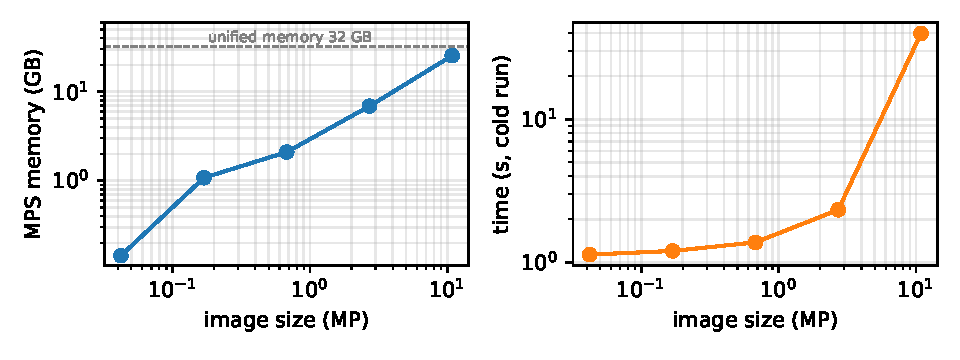
\includegraphics[width=\linewidth]{fig_scaling.pdf}
\caption{Memory (left) and time (right) of one full-resolution CIDNet forward pass versus image size on an Apple M1 (32\,GB), MPS, cold run, on a synthetic image (see text). The last point is 10.8\,MP.}
\label{fig:scaling}
\end{figure}

Table~\ref{tab:cost} compares complete pipelines on the 10.8\,MP image. Tiled inference with 512-pixel tiles takes 14.7\,s with 1.1\,GB, and with 256-pixel tiles 37.7\,s. The low-resolution pipeline with the RGB transform takes 3.9\,s with 2.1\,GB at $1/4$ scale and 3.3\,s with 1.1\,GB at $1/8$: 11 to 13 times faster and 12 to 23 times lighter than the full-resolution pass (42.8\,s, 25.5\,GB), and about 4 times faster than 512-pixel tiling. At $1/2$ scale the bilateral grid becomes large and the transfer takes 10.4\,s, so the whole pipeline (13.4\,s) costs about as much as 512-pixel tiling. The HVI variant is slower in the transfer step (7.3\,s versus 2.2\,s at $1/4$). Part of this is our implementation: the HVI conversions run on the full-resolution tensor with boolean-mask indexing and were not optimized.

\subsection{Ablation ladder}
Table~\ref{tab:ablation} reports the main comparison.
\begin{itemize}
\item \textbf{R1 versus R5/R6.} The bilateral-grid transfer improves fidelity to the teacher over bicubic upsampling by 2.98\,dB ($\times2$), 3.17\,dB ($\times4$) and 3.17\,dB ($\times8$) PSNR for R5 (Wilcoxon $p<10^{-17}$, better on 98\%, 100\% and 100\% of images). Against ground truth, R5 improves LPIPS from 0.333 to 0.188 ($\times2$), from 0.548 to 0.240 ($\times4$) and from 0.729 to 0.273 ($\times8$). Bicubic upsampling is blurry (Fig.~\ref{fig:qual}), so the improvement is visible, but BGU does not reach the teacher: its LPIPS to the ground truth (0.188 at $\times2$) is worse than that of the teacher (0.122).
\item \textbf{R2 and R3.} The gain ratio is the worst method (PSNR to the teacher about 19\,dB): the gain is large in dark regions and multiplies the noise of the full-resolution input, which leads to visibly grainy images and to values above 1. Guided-filter upsampling (R3) is statistically close to bicubic (29.52 against 29.46\,dB at $\times2$) and has a lower SSIM, so R3 does not beat R1; the ladder is not monotone at this rung.
\item \textbf{R5 versus R6 (the main question).} Fitting in HVI does not improve on RGB, even with separately tuned hyper-parameters. PSNR to the teacher is equal at $\times2$ (HVI minus RGB $+0.03$\,dB, $p=0.34$) and slightly higher for HVI at $\times4$ and $\times8$ ($+0.12$\,dB, $p=0.01$; $+0.11$\,dB, $p=0.001$). SSIM to the teacher is lower for HVI by 0.006, 0.010 and 0.012, and LPIPS to the ground truth is higher by 0.011, 0.016 and 0.018 (all $p<10^{-10}$; RGB is better on 86--94\% of images for both metrics). A PSNR gain of about 0.1\,dB together with consistently worse structural and perceptual scores, at a higher cost, does not make HVI the better choice. We interpret this as the absence of a benefit of HVI for this transfer, not as evidence that HVI is harmful in general.
\item \textbf{R4 (tiling).} Tiles of 512 pixels, which for a $600{\times}400$ image means two tiles, are almost identical to the teacher (42.8\,dB, SSIM 0.997). Fidelity decreases quickly for smaller tiles: 35.6\,dB (384), 27.3\,dB (256) and 22.2\,dB (128). Our explanation, which we did not test with a separate experiment, is that the network contains channel-wise attention over the whole spatial extent, so each tile receives different global statistics. Even at 256 pixels, tiling has better SSIM (0.978 against 0.941 for R5 at $\times2$) and better LPIPS to the ground truth (0.131 against 0.188) than the transfer methods, because the network is run on every pixel and removes noise, but lower PSNR (27.3 against 32.4\,dB), consistent with brightness shifts between tiles.
\item \textbf{R7 (gain-aware denoising).} R7 is worse than R5 in PSNR to the teacher at every scale ($-1.96$, $-0.91$ and $-0.50$\,dB at $\times2$, $\times4$, $\times8$; $p<10^{-11}$, better on only 4--19\% of images) and in LPIPS to the ground truth ($+0.086$, $+0.048$, $+0.021$; $p\le0.002$). It improves SSIM to the ground truth only at $\times8$ ($+0.026$, $p<10^{-3}$); at $\times4$ the gain is not significant ($+0.007$, $p=0.095$). Our reading is that the denoised blend removes detail that the teacher keeps, so the output moves away from the teacher even where its noise is reduced; we did not separate these two effects.
\end{itemize}
At $600{\times}400$ resolution, 512-pixel tiles hardly test seam handling; Section~\ref{sec:uhd} tests tiling at 4K.

\begin{figure}[t]
\centering
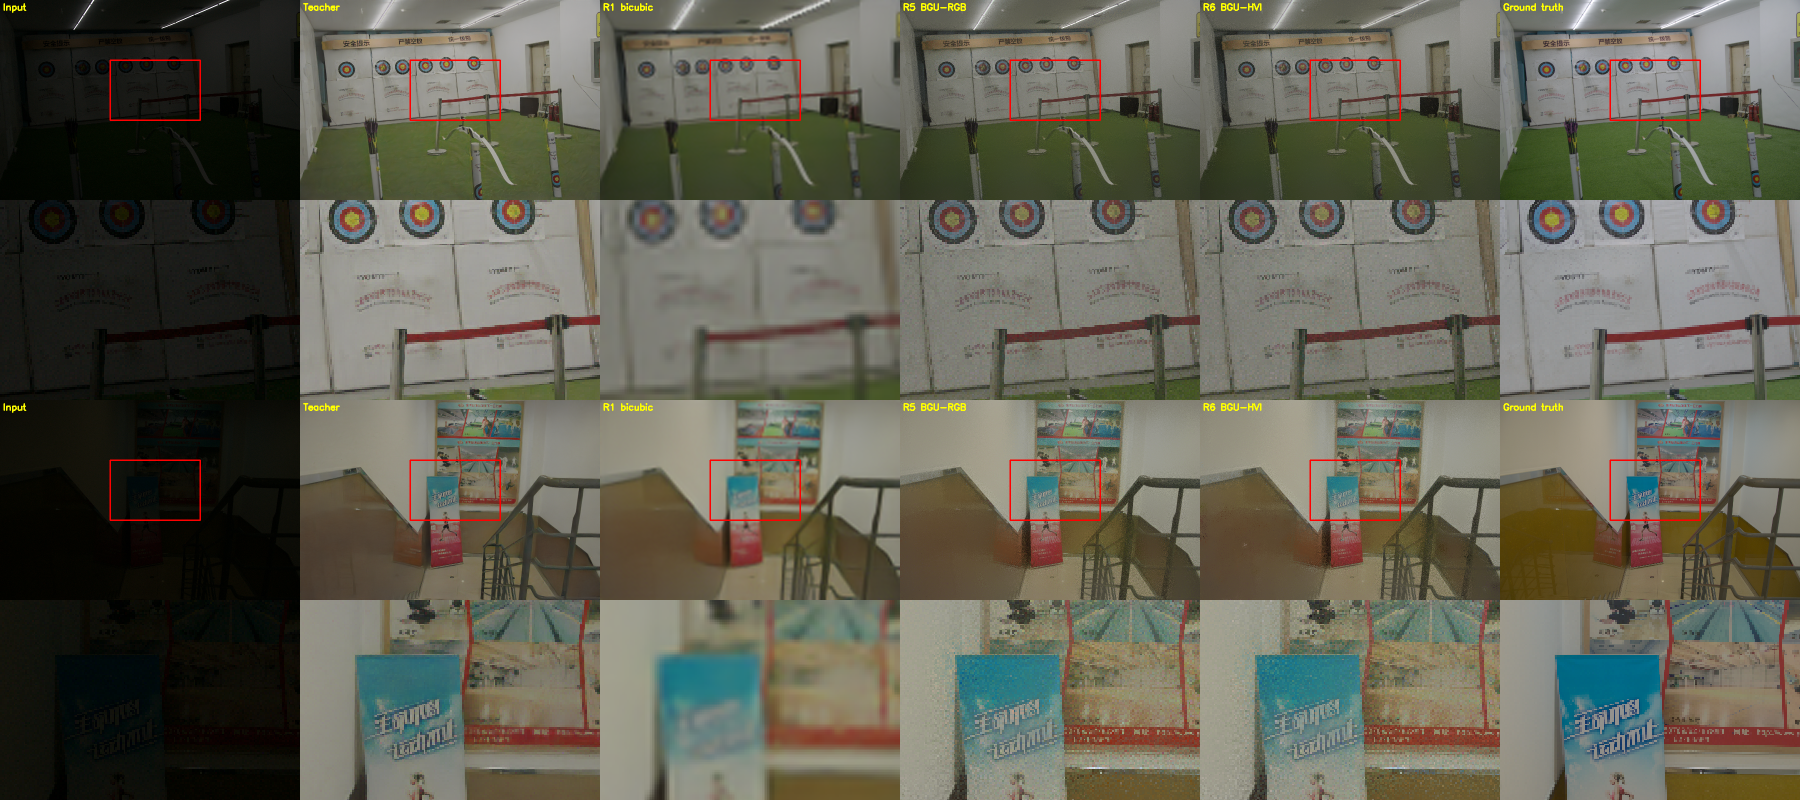
\includegraphics[width=\linewidth]{fig_qual.png}
\caption{Qualitative comparison at $\times4$ downscaling on test images with index 0 and 50 (sorted by name); crops are fixed in advance (red box) and shown with nearest-neighbor magnification. R1 is blurry; R5 and R6 recover edges but reintroduce the grain of the dark input that the teacher removes.}
\label{fig:qual}
\end{figure}

\subsection{Quality--cost trade-off}
Figure~\ref{fig:pareto} combines the two measurements: the horizontal axis is the time of each pipeline on the 10.8\,MP image (Table~\ref{tab:cost}), and the vertical axis is the quality of the same pipeline (same downscaling factor or tile size) on the LOLv2-real test set (Table~\ref{tab:ablation}). Three observations follow. First, BGU-HVI is dominated by BGU-RGB at every operating point: it is slower and not better. Second, 512-pixel tiling dominates the transfer at $1/2$ scale: similar time, much better fidelity and LPIPS. Third, the transfer at $1/4$ and $1/8$ is the only option below about 4\,s, at the price of a clearly visible quality loss. The figure combines quality measured at $600{\times}400$ with cost measured at 10.8\,MP; in particular, at $600{\times}400$ a 512-pixel tiling uses only two tiles, so its quality at megapixel sizes is not measured. The UHD-LL results in Section~\ref{sec:uhd} show that the second observation does not hold at 4K, where tiling quality drops sharply.

\begin{figure}[t]
\centering
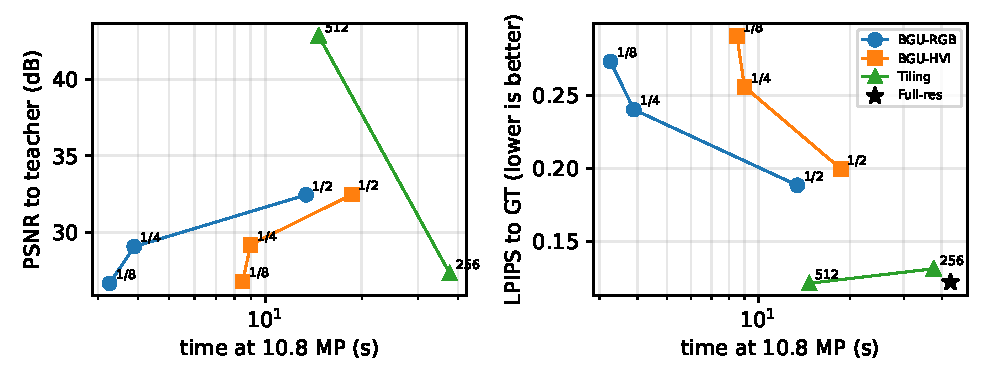
\includegraphics[width=\linewidth]{fig_pareto.pdf}
\caption{Quality versus time. Time: one cold run on a 10.8\,MP image (Table~\ref{tab:cost}). Quality: mean over the LOLv2-real test set at the same downscaling factor (labels $1/s$) or tile size (labels in pixels); left, PSNR to the full-resolution teacher; right, LPIPS to ground truth (the star is the full-resolution network). Quality and cost come from different image sizes; see text.}
\label{fig:pareto}
\end{figure}

\subsection{Real high-resolution images (UHD-LL)}\label{sec:uhd}
Table~\ref{tab:uhd} repeats the comparison on 30 real 4K pairs, with all hyper-parameters frozen; $p$-values are from paired Wilcoxon tests over the 30 images. The full-resolution teacher fits in memory at 8.3\,MP (19.8\,GB on average) and takes 11.7\,s on average.
\begin{itemize}
\item \textbf{Transfer versus bicubic.} R5 is again much closer to the teacher than R1: +3.0, +3.4 and +3.3\,dB PSNR and an SSIM of 0.93 to 0.97 instead of 0.71 to 0.89 at $\times2$, $\times4$ and $\times8$. Fidelity values are higher than on LOLv2-real (38.0\,dB at $\times2$), plausibly because a 4K image is smoother at the scale of a grid cell.
\item \textbf{HVI versus RGB.} R6 is higher than R5 in PSNR to the teacher by only 0.039, 0.034 and 0.020\,dB ($p=3\cdot10^{-4}$, $2\cdot10^{-4}$ and $0.09$); SSIM and the metrics against ground truth differ by about 0.002 or less. The transfer step is 3 to 6 times slower in HVI (e.g.\ 8.8 against 1.8\,s at $\times4$). The conclusion from LOLv2-real therefore carries over to 4K: fitting in HVI brings no practical benefit.
\item \textbf{Tiling.} Tiling is far from the teacher at 4K: 18.8\,dB (512-pixel tiles) and 17.5\,dB (256-pixel tiles) PSNR to the teacher, compared with 42.8 and 27.3\,dB at $600{\times}400$. R5 from a $1/8$ copy (31.9\,dB) is closer to the teacher than 512-pixel tiling on 27 of 30 images, and from a $1/2$ copy on 29 of 30. Tiling also moves the global tone: its PSNR to the ground truth is 13.2\,dB against 17.3\,dB for the teacher. This is consistent with the explanation we gave for small tiles on LOLv2-real, which we have not tested directly: the network uses channel-wise attention over the whole spatial extent, so each tile, which at 4K covers only about 3\% of the image, is enhanced with different global statistics. On this machine, tiling at 4K was also slower than the full-resolution pass (20.5\,s with 512-pixel tiles); its only advantage is memory.
\item \textbf{R7.} R7 is again lower than R5 in fidelity to the teacher ($-0.70$, $-0.33$, $-0.19$\,dB; better on at most 3 of 30 images), but on UHD-LL it improves SSIM ($+0.03$ to $+0.04$) and LPIPS ($-0.026$ to $-0.028$) against the ground truth at every scale ($p<10^{-3}$).
\item \textbf{Ground-truth metrics.} Against ground truth all methods, including the teacher, are poor (PSNR about 17\,dB), because the network was trained on LOLv2 and its output is darker than the UHD-LL references (mean intensity 0.37 against 0.50; darker on 27 of 30 images). This is a domain gap, not a property of the transfer. The teacher also keeps visible noise in dark regions, which R5 and R6 reproduce faithfully (Fig.~\ref{fig:uhd}). Methods that smooth the output, R1 and R7, therefore obtain better SSIM and LPIPS to the ground truth than the teacher itself (R1 at $\times4$: SSIM 0.800 against 0.647). We therefore treat fidelity to the teacher as the primary criterion on UHD-LL, and the metrics against ground truth as secondary.
\end{itemize}

\begin{figure}[t]
\centering
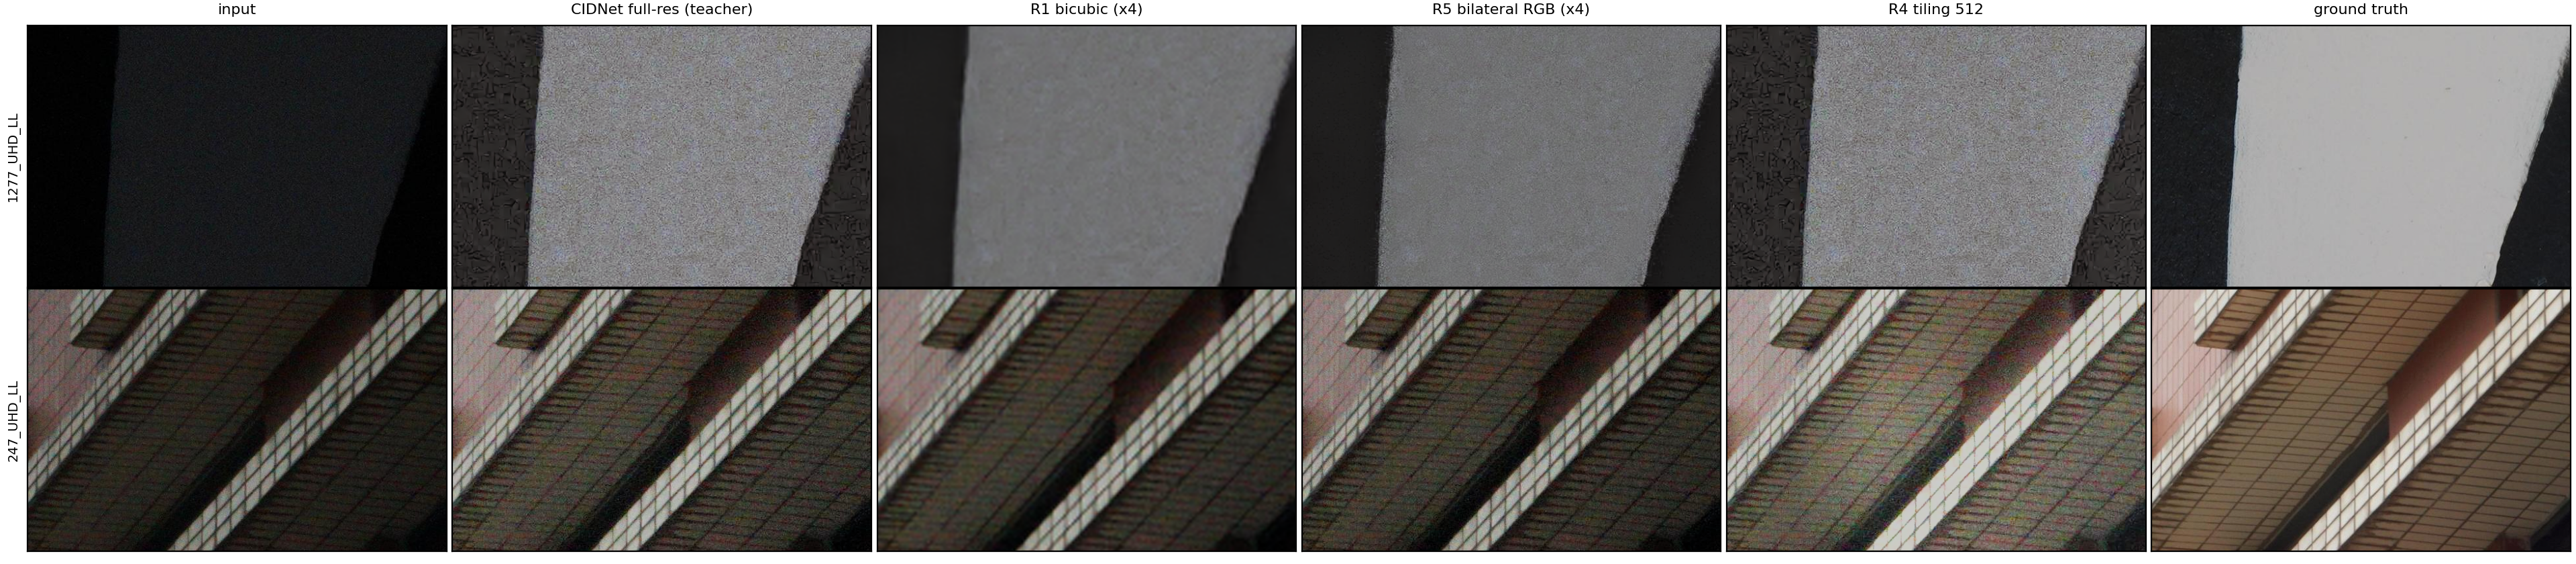
\includegraphics[width=\linewidth]{fig_uhd.png}
\caption{UHD-LL test images 1277 and 247 ($3840{\times}2160$), crop of $640{\times}400$ pixels at a position fixed before running (column 1440, row 720). From left: input, full-resolution teacher, R1 ($\times4$), R5 ($\times4$), tiling with 512-pixel tiles, ground truth. R5 follows the teacher, including its residual noise; R1 is smoother; in the second image tiling is brighter than the teacher.}
\label{fig:uhd}
\end{figure}

\subsection{Discussion}
The transfer methods apply a locally smooth color map to the \emph{full-resolution input}. Everything the network does that is not a smooth color map, notably denoising, cannot be transferred, and the noise of the input is multiplied by the local gain. This is visible in Fig.~\ref{fig:qual} and in the gap in LPIPS and SSIM between R5/R6 and the teacher. It is a structural limit of this family of methods and the reason why they cannot replace the network when the input is very noisy, as in LOLv2-real. R7 shows that a simple fix does not solve this: denoising the input before the transfer also removes detail and moves the output away from the network, even where it moves it closer to a clean reference. The 4K experiment changes the practical recommendation that the LOLv2-real results alone would suggest. On $600{\times}400$ images large tiles look almost free of error because two tiles nearly cover the whole image; on real 4K images tiling is the least faithful option we tested, presumably because the global statistics seen by the network differ from tile to tile. For a device that cannot run the full-resolution pass, our results therefore suggest the RGB transfer from a $1/4$ or $1/8$ copy, which keeps 32 to 34\,dB PSNR to the full-resolution output on UHD-LL and needs only a small network pass; the HVI fit is not worth its extra cost.

%------------------------------------------------------------------
\section{Limitations}\label{sec:limits}
\begin{itemize}
\item \textbf{Size of the real high-resolution test.} UHD-LL results use 30 of the 150 test pairs (a fixed, pre-stated subset), so small differences there should be read with care. We did not evaluate the other UHD-LL pairs or phone photographs.
\item \textbf{Domain gap.} The checkpoint was trained on LOLv2-real; on UHD-LL its output is darker and noisier than the references. Fidelity to the teacher is therefore our main criterion on UHD-LL, and it measures approximation of the network, not image quality.
\item \textbf{One checkpoint, one network.} All results use the LOLv2-real \texttt{best\_PSNR} checkpoint of HVI-CIDNet. We did not test other checkpoints, other networks, or a network trained on high-resolution data.
\item \textbf{Cost measurements} use one machine and a single run per configuration. The 10.8\,MP cost table uses a synthetic image; UHD-LL timings were taken while other jobs shared the machine. Absolute times and memory will differ on other devices; the 4K comparison of tiling and full-resolution time in particular may change on a GPU with more memory.
\item \textbf{Re-implementation.} Our bilateral-grid solver is simplified compared with the original BGU, and hyper-parameters were selected on a small subset. A more careful solver could change the result for R5 and R6, although separate tuning and the 4K test did not change the comparison between them. The selected R7 setting lies at the border of its search grid; other denoisers were not tried.
\item \textbf{Tiling variant.} We tested one tiling scheme (linear-ramp blending, overlap of a quarter tile). Schemes that share global statistics between tiles were not tested and might reduce the tone shift.
\end{itemize}

%------------------------------------------------------------------
\section{Conclusion}
We studied whether a pretrained HVI-CIDNet can be run on a small copy of an image and its result transferred to the large image, to reduce the cost on devices with limited memory. An edge-aware affine transfer on a bilateral grid is much better than bicubic upsampling, both on pseudo-high-resolution LOLv2-real and on real 4K UHD-LL images, and from a $1/4$ or $1/8$ copy it is 11 to 13 times faster than full-resolution inference on a 10.8\,MP image. At 8.3\,MP, where the full-resolution pass still fits in memory on our machine, the gap is smaller (6.3 against 11.7\,s at $1/4$). Fitting the transform in the network's own HVI color space does not improve on fitting it in RGB, and a gain-aware denoising step lowers fidelity to the network. The result that matters most in practice comes from real 4K data: overlapping tiling, which looks almost exact on small benchmark images, drifts far from the full-resolution output at 4K, so the low-resolution RGB transfer is the better cheap pipeline there. Evaluations at benchmark resolution alone would have led to the opposite recommendation. Remaining directions are a transfer that also carries the network's denoising, and tiling that shares global statistics between tiles.

\bibliographystyle{splncs04}
\bibliography{refs}

\end{document}
